% ----------------------------------------------------------------------
% chapters/05_derivative_parser.tex
% ----------------------------------------------------------------------
\chapter{Derivative-Based Parser}
\label{sec:derivative-parser}

Chapter~\ref{sec:derivatives} built a matcher on the Brzozowski
derivative. It returns a Boolean. Chapter~\ref{sec:matching-vs-parsing}
showed that a Boolean is not enough: one expression and one word can
admit several parse trees, and a parser has to return exactly one of
them.

This chapter closes that gap twice, following Sulzmann and Lu
\citep{sulzmannlu2014}. The \emph{direct} construction runs the
derivative sequence forward and rebuilds a tree from it backward. The
\emph{bit-coded} construction builds the tree during the forward pass
and needs no backward pass at all. Both return the POSIX tree, and both
return the same tree.

Each construction gets three sections: its theory, its implementation,
and a worked example checked against the running program. The direct
construction needs little new theory, because
Section~\ref{sec:brzozowski-derivatives} already defined $r\backslash x$,
$n(r)$ and the derivative sequence. The bit-coded construction needs a
full theory section, because it changes the objects the derivative
operates on.

%

\section{From Answer to Evidence}
\label{sec:deriv-parser-motivation}

Take the smallest expression that has a tree worth rebuilding:
$r = a\cdot b$ against $w = \mathtt{ab}$. This example is chosen because
it has exactly \emph{one} parse tree. Ambiguity is the subject of
Section~\ref{sec:deriv-std-worked}; here the question is only whether a
tree can be recovered at all, so an unambiguous case isolates the
mechanism from the choice.

Deriving $a\cdot b$ by $\mathtt{a}$ and then by $\mathtt{b}$ gives
$\varepsilon\cdot b$ and then $\phi\cdot b + \varepsilon$. The last
expression is nullable, so the word matches. That is where
Chapter~\ref{sec:derivatives} stopped.

Now look at what the sequence destroyed. The first step turned the $a$
into $\varepsilon$. The second step turned that $\varepsilon$ into
$\phi$, and turned the $b$ into $\varepsilon$. No consumed character
survives anywhere in the final expression. The tree $(a,b)$ cannot be
read out of it, because the information needed to build it was discarded
one character at a time.

It can be recovered by walking the same sequence backward.
Figure~\ref{fig:two-pass} is the whole idea of the direct construction
in one picture.

\begin{figure}[ht]
\centering
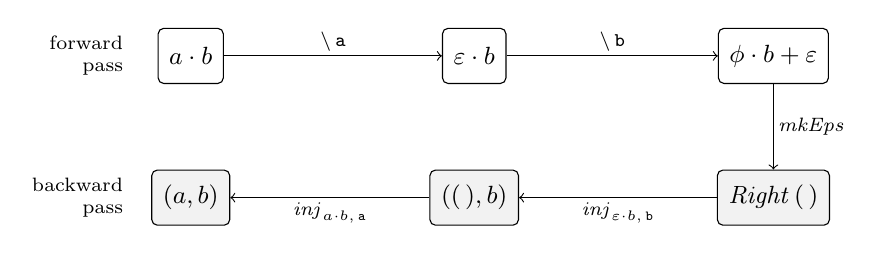
\begin{tikzpicture}[
  expr/.style={draw, rounded corners=2pt, minimum height=7mm,
               font=\small, inner xsep=4pt},
  tree/.style={draw, rounded corners=2pt, minimum height=7mm,
               font=\small, inner xsep=4pt, fill=black!5},
  lbl/.style={font=\scriptsize, inner sep=1.5pt},
]
\node[expr] (r0) at (0,1.8)   {$a\cdot b$};
\node[expr] (r1) at (3.6,1.8) {$\varepsilon\cdot b$};
\node[expr] (r2) at (7.4,1.8) {$\phi\cdot b + \varepsilon$};
\draw[->] (r0) -- node[lbl, above] {$\backslash\,\mathtt{a}$} (r1);
\draw[->] (r1) -- node[lbl, above] {$\backslash\,\mathtt{b}$} (r2);

\node[tree] (v0) at (0,0)   {$(a,b)$};
\node[tree] (v1) at (3.6,0) {$((\,),b)$};
\node[tree] (v2) at (7.4,0) {$\mathit{Right}\,(\,)$};
\draw[->] (v1) -- node[lbl, below] {$\mathit{inj}_{a\cdot b,\,\mathtt{a}}$} (v0);
\draw[->] (v2) -- node[lbl, below] {$\mathit{inj}_{\varepsilon\cdot b,\,\mathtt{b}}$} (v1);

\draw[->] (r2) -- node[lbl, right] {$\mathit{mkEps}$} (v2);

\node[lbl, anchor=east, align=right] at (-0.8,1.8) {forward\\pass};
\node[lbl, anchor=east, align=right] at (-0.8,0)   {backward\\pass};
\end{tikzpicture}
\caption{The direct construction on $a\cdot b$ against \texttt{"ab"}.
The top row is the derivative sequence of
Section~\ref{sec:brzozowski-derivatives}. $\mathit{mkEps}$ turns at the
end and builds a tree for the empty word. Each $\mathit{inj}$ step
undoes one derivative and puts back the character that step consumed.
Every expression in the top row must stay in memory until the step
below it has run.}
\label{fig:two-pass}
\end{figure}

The figure names the two functions this chapter has to define. At the
right-hand end, $\mathit{mkEps}$ builds a tree for the empty word. That
is all the final expression can justify, since nothing remains to be
matched. Each $\mathit{inj}$ step then moves one column to the left and
reinserts one character. After the first step the tree is $((\,),b)$.
The $b$ is back in place, and $(\,)$ holds open the position where the
$a$ belongs. After the second step that placeholder has become $a$ and
the tree is complete.

The forward row is unchanged from Chapter~\ref{sec:derivatives}. This
chapter adds only the bottom row.

\subsection{Which Tree}
\label{sec:posix-longest-leftmost}

The $a\cdot b$ example has one tree, so it does not say which tree a
parser should return when there are several. The chapter's running
example does. It is $r_1$ from
Section~\ref{sec:disambiguation-problem}:

\[
r_1 = (a+ab)(b+\varepsilon), \qquad w = \mathtt{ab},
\]

with the two candidates
$v_1 = (\mathit{Right}(a,b), \mathit{Right}(\,))$ and
$v_1' = (\mathit{Left}\ a, \mathit{Left}\ b)$.

Both parsers in this chapter return $v_1$, because both implement POSIX.
The standard states the rule in one sentence: consistent with the whole
match being the longest of the leftmost matches, each subpattern, from
left to right, shall match the longest possible string
\citep[Section~9.1]{posix_ere}.

Read that against $r_1$. The leftmost subpattern is $a+ab$. Of the two
splits of $\mathtt{ab}$, only one lets that subpattern match two
characters. So $a+ab$ takes $\mathtt{ab}$ through its right alternative.
That leaves nothing for $b+\varepsilon$, which must then take
$\varepsilon$, also its right alternative. Two right choices give $v_1$.

Greedy, the other policy named in
Section~\ref{sec:disambiguation-problem}, prefers the earlier
alternative at each choice and so selects $v_1'$. This chapter does not
formalize either ordering. What matters is that the target is a definite
tree, that it is $v_1$, and that neither construction ever builds both
candidates and compares them. Each makes one local decision, and the two
theory sections below say exactly where that decision sits.

%

\section{Tree Construction}
\label{sec:core-algorithm}

\subsection{The Empty-Word Tree}
\label{sec:mkeps-theory}

$\mathit{mkEps}$ takes a nullable expression and returns a parse tree
for the empty word. It recurses on the structure of the expression:

\begin{equation}\label{eq:mkeps}
\begin{aligned}
\mathit{mkEps}_{\varepsilon} &= () &&(\mathsf{E}_{\varepsilon}) \\
\mathit{mkEps}_{r^{*}} &= [\,] &&(\mathsf{E}_{*}) \\
\mathit{mkEps}_{r_1 r_2} &= (\mathit{mkEps}_{r_1}, \mathit{mkEps}_{r_2})
  &&(\mathsf{E}_{\mathrm{seq}}) \\
\mathit{mkEps}_{r_1+r_2} &=
  \begin{cases}
    \mathit{Left}\ \mathit{mkEps}_{r_1} & \varepsilon \in L(r_1) \\
    \mathit{Right}\ \mathit{mkEps}_{r_2} & \text{otherwise}
  \end{cases}
  &&\begin{array}{l}(\mathsf{E}_{+}^{L}) \\ (\mathsf{E}_{+}^{R})\end{array}
\end{aligned}
\end{equation}

The rule names continue the scheme of
Section~\ref{sec:brzozowski-derivatives}. Every derivation below cites
them and states the binding of $r_1$ and $r_2$, since which
subexpression each stands for is what decides the case.

Three of the four rules are forced. $\varepsilon$ has one tree. A star
matching the empty word took zero iterations, which is
$\mathsf{T}_{*}^{0}$ of Equation~\eqref{eq:typing-rules} read backward.
A concatenation matches empty only when both factors do, by
$\mathsf{N}_{\mathrm{seq}}$, so both halves of the pair exist. There is
no rule for a literal or for $\emptyset$, because neither is ever
nullable and the function is never called on one.

The fourth rule is the decision. When both disjuncts are nullable, both
match the empty word and both consume nothing. "Longest possible string"
cannot separate them, so POSIX falls back on position and prefers the
left. That is the $\varepsilon\in L(r_1)$ guard.

The guard is a test, not a comparison. $\mathsf{E}_{+}^{L}$ and
$\mathsf{E}_{+}^{R}$ are never both applicable, because the case split
looks only at $r_1$. If the left disjunct is nullable,
$\mathsf{E}_{+}^{L}$ fires and the right disjunct is never examined.
Sulzmann and Lu prove that deciding this way yields the POSIX tree
\citep{sulzmannlu2014}.

\subsection{Reinserting a Character}
\label{sec:inj-theory}

$\mathit{inj}$ inverts one derivative step. Given a parse tree of
$r\backslash x$, it returns a parse tree of $r$ with $x$ put back:

\begin{equation}\label{eq:inj}
\begin{aligned}
\mathit{inj}_{x \backslash x}() &= x &&(\mathsf{I}_{\mathrm{lit}}) \\
\mathit{inj}_{(r_1+r_2) \backslash x}(\mathit{Left}\ v_1)
  &= \mathit{Left}\ (\mathit{inj}_{r_1 \backslash x}\ v_1)
  &&(\mathsf{I}_{+}^{L}) \\
\mathit{inj}_{(r_1+r_2) \backslash x}(\mathit{Right}\ v_2)
  &= \mathit{Right}\ (\mathit{inj}_{r_2 \backslash x}\ v_2)
  &&(\mathsf{I}_{+}^{R}) \\
\mathit{inj}_{r^{*} \backslash x}(v, vs)
  &= (\mathit{inj}_{r \backslash x}\ v) : vs
  &&(\mathsf{I}_{*}) \\
\mathit{inj}_{(r_1 r_2) \backslash x}(v_1, v_2)
  &= (\mathit{inj}_{r_1 \backslash x}\ v_1,\ v_2)
  &&(\mathsf{I}_{\mathrm{seq}}),\ n(r_1) = \mathrm{false} \\
\mathit{inj}_{(r_1 r_2) \backslash x}(\mathit{Left}(v_1, v_2))
  &= (\mathit{inj}_{r_1 \backslash x}\ v_1,\ v_2)
  &&(\mathsf{I}_{\mathrm{seq}}^{L}),\ n(r_1) = \mathrm{true} \\
\mathit{inj}_{(r_1 r_2) \backslash x}(\mathit{Right}\ v_2)
  &= (\mathit{mkEps}_{r_1},\ \mathit{inj}_{r_2 \backslash x}\ v_2)
  &&(\mathsf{I}_{\mathrm{seq}}^{R}),\ n(r_1) = \mathrm{true}
\end{aligned}
\end{equation}

The first four rules are direct. A literal was derived to $\varepsilon$,
so the only tree it can receive is $()$, and the character goes back. An
alternation was derived on both sides, so the incoming tag says which
side to descend into. A star was derived to
$(r\backslash x)\cdot r^{*}$, so the incoming tree is a pair whose first
component belongs to the iteration in progress.

The three concatenation rules need the derivative rule they invert.
Section~\ref{sec:brzozowski-derivatives} gave two cases. When $n(r_1)$
is false, the derivative is $(r_1\backslash x)\, r_2$ and no alternation
appears. When $n(r_1)$ is true, the derivative joins that same term with
$r_2\backslash x$ under a \emph{fresh} $+$. That fresh $+$ tags the
incoming tree, and the tag says which branch was taken:

\begin{center}
\begin{tabular}{@{}ll>{\raggedright\arraybackslash}p{6.4cm}@{}}
\hline
Incoming tree & Rule & What the derivative did \\
\hline
$(v_1,v_2)$ & $\mathsf{I}_{\mathrm{seq}}$ &
  $r_1$ was not nullable. No $+$ was introduced, and the derivative went
  straight into $r_1$. \\[2pt]
$\mathit{Left}(v_1,v_2)$ & $\mathsf{I}_{\mathrm{seq}}^{L}$ &
  $r_1$ was nullable, and the derivative still continued inside
  $r_1$. \\[2pt]
$\mathit{Right}\ v_2$ & $\mathsf{I}_{\mathrm{seq}}^{R}$ &
  $r_1$ was nullable and the derivative skipped it. Nothing of $r_1$ was
  consumed, so its half of the pair has to be synthesized by
  $\mathit{mkEps}_{r_1}$. \\
\hline
\end{tabular}
\end{center}

The last row calls $\mathit{mkEps}$ a second time, in the middle of the
backward pass. Section~\ref{sec:bitcoded-optimization-theory} removes
that call.

\subsection{The Parser}
\label{sec:deriv-parse-theory}

The two functions compose into one recursion. It applies
$\mathit{mkEps}$ once, at the end of the input, and $\mathit{inj}$ once
per character on the way back:

\begin{equation}\label{eq:parse}
\begin{aligned}
\mathit{parse}(r, \varepsilon) &= \mathit{mkEps}_r
  \qquad (\text{if } \varepsilon \in L(r)) \\
\mathit{parse}(r, xw) &= \mathit{inj}_{r \backslash x}(\mathit{parse}(r \backslash x, w))
\end{aligned}
\end{equation}

If the expression reached at the end of the input is not nullable, no
parse tree exists and parsing fails.

\subsection{No Simplification}
\label{sec:deriv-no-simp}

One rule constrains the forward pass: it must not simplify.

Section~\ref{sec:brzozowski-derivatives} applied the identities of
Equation~\eqref{eq:simp-identities} after every derivative step, and for
a Boolean matcher that is safe. Simplification replaces $r_i$ by a
language-equivalent expression, and language equivalence is all a
Boolean answer depends on.

The backward pass depends on more. $\mathit{inj}_{r\backslash x}$ is
indexed by $r$, and its case split reads $r$'s shape: whether the node
is a $\mathit{Seq}$, and whether that $\mathit{Seq}$'s left factor is
nullable. $\mathsf{S}_{2}$ alone, which rewrites $\varepsilon\cdot r$ to
$r$, deletes exactly such a node. The backward pass would then meet an
expression that is not the one its tree came from.

So the direct construction pays for the tree in expression size. The
bit-coded construction does not, and
Section~\ref{sec:simplification-rules-theory} explains why it is free to
simplify.

%

\section{Implementation: \texttt{deriv\_std}}
\label{sec:derivative-parser-inj-rust}

\subsection{What the Parser Needs}
\label{sec:deriv-std-module-map}

The direct parser is four functions over the \texttt{Regex} enum of
Figure~\ref{fig:regex-enum}, plus a driver. Each transcribes one
equation, with the case split of the equation becoming the arms of a
\texttt{match} and the recursion becoming recursion.

\begin{center}
\begin{tabular}{@{}lll@{}}
\hline
Function & Transcribes & Also used by \\
\hline
\texttt{nullable} & Equation~\eqref{eq:nullability} & every parser and matcher \\
\texttt{deriv} & Equation~\eqref{eq:derivative} & \texttt{match\_deriv} \\
\texttt{mk\_eps} & Equation~\eqref{eq:mkeps} & \texttt{pderiv\_std} \\
\texttt{inject} & Equation~\eqref{eq:inj} & nothing else \\
\hline
\end{tabular}
\end{center}

The first two are Chapter~\ref{sec:derivatives}'s and are unchanged
here. The last two are this chapter's.

\texttt{simplify} is absent from the table, and that absence is
Section~\ref{sec:deriv-no-simp}'s rule enforced by the module's imports:
the direct parser does not import it, so no forward step can simplify by
accident. The two matchers of Chapter~\ref{sec:derivatives} do import
it.

\subsection{\texttt{mk\_eps}}
\label{sec:mk-eps-impl}

Equation~\eqref{eq:mkeps} has four clauses, one per nullable construct.
Figure~\ref{fig:mkeps-rust} is the whole function.

\begin{figure}[H]
\begin{verbatim}
pub fn mk_eps(r: &Regex) -> ParseTree {
    match r {
        Regex::Eps => ParseTree::Empty,
        Regex::Star(_) => ParseTree::Star(Vec::new()),
        Regex::Seq(r1, r2) => {
            let v1 = mk_eps(r1);
            let v2 = mk_eps(r2);
            ParseTree::Pair(Box::new(v1), Box::new(v2))
        }
        Regex::Alt(r1, r2) => {
            if nullable(r1) {
                ParseTree::Left(Box::new(mk_eps(r1)))
            } else {
                ParseTree::Right(Box::new(mk_eps(r2)))
            }
        }
        Regex::Lit(c) => panic!("mk_eps called on Lit('{}')", c),
        Regex::Phi => panic!("mk_eps called on Phi"),
    }
}
\end{verbatim}
\caption{\texttt{mk\_eps}, transcribing Equation~\eqref{eq:mkeps}. The
first four arms are $\mathsf{E}_{\varepsilon}$, $\mathsf{E}_{*}$,
$\mathsf{E}_{\mathrm{seq}}$ and the
$\mathsf{E}_{+}^{L}$/$\mathsf{E}_{+}^{R}$ pair, in that order.}
\label{fig:mkeps-rust}
\end{figure}

\paragraph{Why it is written this way.}
Three decisions in this function are worth naming.

The expression is borrowed, not consumed. \texttt{mk\_eps} only reads
$r$, and the same $r$ is read again by \texttt{inject} later in the
backward pass, so a \texttt{\&Regex} is the only signature that works.
The tree it returns is freshly built and owned.

The \texttt{Alt} arm is the entire POSIX decision, and it is one
\texttt{if}. Nothing compares the two branches. \texttt{nullable(r1)} is
evaluated, and \texttt{r2} is touched only when it comes back false.
That is $\mathsf{E}_{+}^{L}$'s guard, $\varepsilon\in L(r_1)$, with no
appeal to lengths, because at the empty word there are no lengths to
compare.

The last two arms encode a precondition. Equation~\eqref{eq:mkeps} has
no clause for $\phi$ or for a literal, because neither is nullable and
the function is never called on one. A Rust \texttt{match} on an enum
must cover every variant, so the transcription has to write something.
It writes \texttt{panic!}, which states the precondition rather than
working around it. The alternative is to invent a tree and return it,
and a wrong parse tree that is well formed is exactly what the agreement
tests of Chapter~\ref{sec:evaluation} cannot detect, because they
compare parsers against each other and two guesses can agree.

\subsection{\texttt{inject}: The Direct Rules}
\label{sec:inject-impl}

\texttt{inject(r, l, v)} carries three arguments because $\mathit{inj}$
is indexed by an expression and a character. The tree alone does not
determine the rule.

Section~\ref{sec:inj-theory} split Equation~\eqref{eq:inj} into four
direct rules and three concatenation rules.
Figure~\ref{fig:inject-rust} is the first group, with the concatenation
arm held back for Figure~\ref{fig:inject-seq-rust}.

\begin{figure}[H]
\begin{verbatim}
pub fn inject(r: &Regex, l: char, v: ParseTree) -> ParseTree {
    match r {
        Regex::Lit(c) => {
            assert!(*c == l);
            assert!(matches!(v, ParseTree::Empty));
            ParseTree::Char(l)
        }

        Regex::Alt(r1, r2) => match v {
            ParseTree::Left(v1) =>
                ParseTree::Left(Box::new(inject(r1, l, *v1))),
            ParseTree::Right(v2) =>
                ParseTree::Right(Box::new(inject(r2, l, *v2))),
            _ => panic!("inject/Alt: want Left|Right, got {:?}", v),
        },

        Regex::Star(r1) => match v {
            ParseTree::Pair(v1, vs) => {
                let mut iterations = vec![inject(r1, l, *v1)];
                if let ParseTree::Star(rest) = *vs {
                    iterations.extend(rest);
                }
                ParseTree::Star(iterations)
            }
            _ => panic!("inject/Star: want Pair, got {:?}", v),
        },

        Regex::Seq(r1, r2) => { /* see the next figure */ }

        Regex::Eps => panic!("inject called on Eps"),
        Regex::Phi => panic!("inject called on Phi"),
    }
}
\end{verbatim}
\caption{\texttt{inject}, with the literal, alternation and star arms
transcribing $\mathsf{I}_{\mathrm{lit}}$, $\mathsf{I}_{+}^{L}$,
$\mathsf{I}_{+}^{R}$ and $\mathsf{I}_{*}$ of
Equation~\eqref{eq:inj}.}
\label{fig:inject-rust}
\end{figure}

\paragraph{Why it is written this way.}
The function matches on \texttt{r} at the top level and on \texttt{v}
inside each arm, and that order is the definition's order.
Equation~\eqref{eq:inj} indexes every rule by the expression first, and
the tree tag then selects among the rules that expression allows.
Matching on \texttt{v} first would not work, since a \texttt{Left} tag
means one thing under an alternation and something else under a nullable
concatenation.

The literal arm is two assertions and a constructor. The assertions say
what $\mathsf{I}_{\mathrm{lit}}$ leaves implicit in its indexing: the
character being reinserted is the literal's own, and the tree handed in
is the $()$ that $\mathsf{D}_{\mathrm{lit}}$ produced. Neither can fail
if the tree came from this expression's own derivative sequence.

The star arm is where the parse tree's list representation shows. The
derivative turned $r^{*}$ into $(r\backslash l)\cdot r^{*}$, so the
incoming tree is a \texttt{Pair}: the iteration in progress on the left,
and the iterations already recovered on the right. The code injects into
the first, then flattens the second onto it with
\texttt{iterations.extend(rest)}, which is
$(\mathit{inj}\ v) : vs$ written for a \texttt{Vec}. The \texttt{if let}
guards the case where \texttt{vs} is not a \texttt{Star}, which cannot
arise from a well-formed derivative and yields an empty tail if it
somehow did.

\subsection{\texttt{inject}: Concatenation}
\label{sec:inject-seq-impl}

Figure~\ref{fig:inject-seq-rust} is the arm held back above. It is the
three-row table of Section~\ref{sec:inj-theory}.

\begin{figure}[H]
\begin{verbatim}
Regex::Seq(r1, r2) => {
    if !nullable(r1) {
        match v {
            ParseTree::Pair(v1, v2) => ParseTree::Pair(
                Box::new(inject(r1, l, *v1)), v2),
            _ => panic!("inject/Seq: want Pair, got {:?}", v),
        }
    } else {
        match v {
            ParseTree::Left(vp) => match *vp {
                ParseTree::Pair(v1, v2) => ParseTree::Pair(
                    Box::new(inject(r1, l, *v1)), v2),
                o => panic!("inject/SeqL: want Pair, got {:?}", o),
            },
            ParseTree::Right(v2) => ParseTree::Pair(
                Box::new(mk_eps(r1)),
                Box::new(inject(r2, l, *v2))),
            _ => panic!("inject/Seq: want Left|Right, got {:?}", v),
        }
    }
}
\end{verbatim}
\caption{The concatenation arm of \texttt{inject}, transcribing
$\mathsf{I}_{\mathrm{seq}}$, $\mathsf{I}_{\mathrm{seq}}^{L}$ and
$\mathsf{I}_{\mathrm{seq}}^{R}$. The three reachable arms appear in the
order of Section~\ref{sec:inj-theory}'s table.}
\label{fig:inject-seq-rust}
\end{figure}

\paragraph{Why it is written this way.}
The outer \texttt{if} is the side condition $n(r_1)$ and the inner
\texttt{match} reads the tag the derivative left behind. The two are
separate tests because the rules are indexed on two separate things: the
expression decides whether a fresh $+$ was introduced at all, and only
then does the tree's tag mean anything.

Calling \texttt{nullable(r1)} here is a recomputation. The forward pass
already evaluated it at this node, when
$\mathsf{D}_{\mathrm{seq}}^{\,n}$ was chosen over
$\mathsf{D}_{\mathrm{seq}}$, and discarded the answer. Caching it would
mean carrying a second structure alongside the expression sequence,
which is the kind of bookkeeping
Section~\ref{sec:bitcoded-optimization-theory} avoids by not having a
backward pass at all.

The ownership split follows the data flow. \texttt{r} is borrowed and
only read; \texttt{v} is taken by value, because the tree is taken apart
and rebuilt. That is what lets the \texttt{Left} arm write
\texttt{match *vp}, moving the tree out of its \texttt{Box} to
destructure it. It is also what lets both matching arms hand
\texttt{v2} straight into the new \texttt{Pair} with no copy: in
Equation~\eqref{eq:inj} the component $v_2$ appears unchanged on the
right-hand side of $\mathsf{I}_{\mathrm{seq}}$ and
$\mathsf{I}_{\mathrm{seq}}^{L}$, and in Rust an unchanged component is
a move.

The \texttt{Right} arm is the only one that builds something new.
$\mathsf{I}_{\mathrm{seq}}^{R}$ has nothing to reuse for $r_1$'s half of
the pair, because the derivative skipped $r_1$ entirely and consumed
none of it, so \texttt{mk\_eps(r1)} synthesizes that half. This is the
second \texttt{mk\_eps} call of the backward pass, and the one
Section~\ref{sec:bderiv-theory}'s $\mathit{fuse}$ moves into the forward
pass.

\subsection{Two Drivers}
\label{sec:recursive-vs-loop}

Equation~\eqref{eq:parse} is a recursion.
Figure~\ref{fig:deriv-std-drivers-rust} transcribes it twice.

\begin{figure}[H]
\begin{verbatim}
fn parse_recursive_helper(r: &Regex, input: &str)
    -> Option<ParseTree>
{
    let mut chars = input.chars();
    match chars.next() {
        None => {
            if nullable(r) { Some(mk_eps(r)) } else { None }
        }
        Some(l) => {
            let rest: String = chars.collect();
            let r_deriv = deriv(r, l);
            let subtree = parse_recursive_helper(&r_deriv, &rest)?;
            Some(inject(r, l, subtree))
        }
    }
}

pub fn parse_deriv_std_loop(input: &str, r: &Regex)
    -> Option<ParseTree>
{
    let chars: Vec<char> = input.chars().collect();
    let n = chars.len();

    let mut expressions = Vec::with_capacity(n + 1);
    expressions.push(r.clone());

    for &c in chars.iter() {
        let current = expressions.last().unwrap();
        let next = deriv(current, c);
        expressions.push(next);
    }

    let final_r = expressions.last().unwrap();
    if !nullable(final_r) {
        return None;
    }

    let mut tree = mk_eps(expressions.last().unwrap());
    for i in (0..n).rev() {
        tree = inject(&expressions[i], chars[i], tree);
    }

    Some(tree)
}
\end{verbatim}
\caption{The two entry points. The recursive one is
Equation~\eqref{eq:parse} read literally. The loop one materializes
Figure~\ref{fig:two-pass}'s top row as a \texttt{Vec<Regex>} and then
walks it backward.}
\label{fig:deriv-std-drivers-rust}
\end{figure}

The recursive driver never stores the top row. The call stack is the top
row: each frame holds its own \texttt{r} and \texttt{l}, the descent runs
to the end of the input, and \texttt{inject} runs as the stack unwinds.
The \texttt{?} operator propagates a failed match, so a \texttt{None}
from the recursive call returns immediately and no injection is
attempted.

The loop driver stores the top row explicitly, then indexes it backward
with \texttt{(0..n).rev()}.

The algorithm is the same. The resource behaviour is not. A thread's
stack in Rust is a fixed allocation made when the thread starts, while a
\texttt{Vec} grows on the heap. The recursive driver overflows the stack
on input the loop driver handles without difficulty.
Section~\ref{sec:stack-depth} measures where the difference begins.

\subsection{Trees and Flattening}
\label{sec:parsetree-and-flatten}

Both drivers return an \texttt{Option} over the \texttt{ParseTree} of
Section~\ref{sec:parse-trees-as-evidence}. Every parser in this thesis
produces that one type, which is what lets the agreement tests compare
outputs directly.

\texttt{flatten} is kept out of tree construction so that it can serve
as an independent check. It discards every tag and every pair boundary
and returns the concatenated literals. A successful parse of $w$ must
flatten back to $w$, whatever the disambiguation policy was. Every
diagnostic report prints the tree and its flattening side by side for
that reason.

%

\section{Worked Example: \texttt{deriv\_std}}
\label{sec:deriv-std-worked}

This section runs $r_1 = (a+ab)(b+\varepsilon)$ against $\mathtt{ab}$
through the construction, and checks each step against the tool's own
report:

\begin{verbatim}
cargo run -- parse "(a|ab)(b|)" "ab" --parser deriv_std_rec --diag 3
\end{verbatim}

where \texttt{"(a|ab)(b|)"} is $r_1$ in the surface syntax of
Section~\ref{sec:frontend-parsing}, with $\varepsilon$ spelled as an
empty right alternative. The tool's Unicode is transliterated to ASCII
below ($\partial$ as \texttt{d}, $\varepsilon$ as \texttt{epsilon},
$\phi$ as \texttt{phi}), and long lines are wrapped; the full report is
Appendix~\ref{app:report-deriv-std-match}.

\subsection{Forward Pass}
\label{sec:deriv-std-worked-forward}

Two derivative steps consume the input:

\begin{equation}\label{eq:dp-4}
\begin{aligned}
r_1 &\xrightarrow{\ a\ } (\varepsilon+\varepsilon b)(b+\varepsilon)
    &&\mathsf{D}_{\mathrm{seq}},\ r = a+ab,\ s = b+\varepsilon,\ n(r) = \mathrm{false} \\
    &\xrightarrow{\ b\ } (\phi+(\phi b+\varepsilon))(b+\varepsilon)
       + (\varepsilon+\phi)
    &&\mathsf{D}_{\mathrm{seq}}^{\,n},\ r = \varepsilon+\varepsilon b,\ n(r) = \mathrm{true}
\end{aligned}
\end{equation}

The two steps take different cases of the same rule. The binding is
what changes. Initially the left operand is $a+ab$, which is not
nullable. After one character it is $\varepsilon+\varepsilon b$, which
is nullable by $\mathsf{N}_{+}$ and $\mathsf{N}_{\varepsilon}$. That is
what adds the summand $(\varepsilon+\phi)$ at the second step, and that
summand is what makes the whole expression nullable.

The report confirms both the rule and the full expression:

\begin{verbatim}
Step 1: d(r0, 'a')
  rule: d(r1.r2, 'a')  [nullable(r1)=false]
       = d(r1, 'a').r2
r1 = Seq(Alt(Eps, Seq(Eps, Lit('b'))), Alt(Lit('b'), Eps))
  nullable(r1) = true  [OK] position 1 matched

Step 2: d(r1, 'b')
  rule: d(r1.r2, 'b')  [nullable(r1)=true]
       = d(r1, 'b').r2  +  d(r2, 'b')
r2 = Alt(Seq(Alt(Phi, Alt(Seq(Phi, Lit('b')), Eps)), Alt(Lit('b'),
  Eps)), Alt(Eps, Phi))
  nullable(r2) = true  [OK] position 2 matched
\end{verbatim}

Step 1 also makes Section~\ref{sec:deriv-no-simp} concrete. The
\texttt{Eps} inside \texttt{Seq(Eps, Lit('b'))} is exactly the node
$\mathsf{S}_{2}$ would delete. It is printed, so it was kept, and the
backward pass will read it.

\subsection{The Empty-Word Tree}
\label{sec:deriv-std-worked-mkeps}

Step 2 introduced a fresh \texttt{Alt} at the top of $r_2$. Both of its
disjuncts are nullable, so this is the case
Section~\ref{sec:mkeps-theory} singled out.

Write $X = \phi + (\phi b + \varepsilon)$ and $Y = b + \varepsilon$ for
the two factors of the left disjunct:

\begin{equation}\label{eq:dp-mkeps-derivation}
\begin{aligned}
\mathit{mkEps}_{r_2}
&= \mathit{Left}\ \mathit{mkEps}_{X\,Y}
&&\mathsf{E}_{+}^{L},\ r_1 = X\,Y,\ r_2 = \varepsilon+\phi \\
&= \mathit{Left}\ (\mathit{mkEps}_{X}, \mathit{mkEps}_{Y})
&&\mathsf{E}_{\mathrm{seq}},\ r_1 = X,\ r_2 = Y \\
&= \mathit{Left}\ (\mathit{Right}\ \mathit{mkEps}_{\phi b+\varepsilon},\
   \mathit{Right}\ \mathit{mkEps}_{\varepsilon})
&&\mathsf{E}_{+}^{R}\ \text{twice},\ \varepsilon \notin L(\phi),\
   \varepsilon \notin L(b) \\
&= \mathit{Left}\ (\mathit{Right}\ \mathit{Right}\ (),\ \mathit{Right}\ ())
&&\mathsf{E}_{+}^{R},\ \mathsf{E}_{\varepsilon}
\end{aligned}
\end{equation}

The report prints the first line on its own, because it is the only line
with a choice in it:

\begin{verbatim}
mkEps(r2):
  mkEps(r1 + r2): nullable(r1)=true -> Left(mkEps(r1))
v2 = Left (Right Right (), Right ())
\end{verbatim}

One decision was made and three cases followed from it. The outer
$\mathsf{E}_{+}^{L}$ commits to the summand that came from continuing
inside $a+ab$. After that, $\mathsf{E}_{\mathrm{seq}}$ has no choice,
and the two $\mathsf{E}_{+}^{R}$ steps take right branches only because
their left operands, $\phi$ and $b$, are not nullable.

\subsection{The Two Injections}
\label{sec:deriv-std-worked-inject}

The backward pass runs twice. The first injection undoes the
$\mathtt{b}$ step. Write $X' = \varepsilon+\varepsilon b$ for the left
factor of $r_1$:

\begin{equation}\label{eq:dp-inj-b}
\begin{aligned}
\mathit{inj}_{r_1\backslash \mathtt{b}}(v_2)
&= (\mathit{inj}_{X'\backslash \mathtt{b}}(\mathit{Right}\ \mathit{Right}\ ()),\
    \mathit{Right}\ ())
&&\mathsf{I}_{\mathrm{seq}}^{L},\ n(X') = \mathrm{true} \\
&= (\mathit{Right}\ \mathit{inj}_{(\varepsilon b)\backslash \mathtt{b}}(\mathit{Right}\ ()),\
    \mathit{Right}\ ())
&&\mathsf{I}_{+}^{R},\ r_2 = \varepsilon b \\
&= (\mathit{Right}\ (\mathit{mkEps}_{\varepsilon},\
    \mathit{inj}_{b\backslash \mathtt{b}}()),\ \mathit{Right}\ ())
&&\mathsf{I}_{\mathrm{seq}}^{R},\ n(\varepsilon) = \mathrm{true} \\
&= (\mathit{Right}\ ((\,), b),\ \mathit{Right}\ ())
&&\mathsf{E}_{\varepsilon},\ \mathsf{I}_{\mathrm{lit}}
\end{aligned}
\end{equation}

Two rows of Section~\ref{sec:inj-theory}'s table appear here. The first
line is $\mathsf{I}_{\mathrm{seq}}^{L}$ undoing the \texttt{Left} that
$\mathit{mkEps}$ had just produced. The third line is
$\mathsf{I}_{\mathrm{seq}}^{R}$: the derivative had skipped the nullable
$\varepsilon$ and jumped into $b$, so $\varepsilon$'s half of the pair
is synthesized by $\mathit{mkEps}$ and not recovered.

The second injection undoes the $\mathtt{a}$ step:

\begin{equation}\label{eq:dp-inj-a}
\begin{aligned}
\mathit{inj}_{r_0\backslash \mathtt{a}}(v_1)
&= (\mathit{inj}_{(a+ab)\backslash \mathtt{a}}(\mathit{Right}\ ((\,),b)),\
    \mathit{Right}\ ())
&&\mathsf{I}_{\mathrm{seq}},\ n(a+ab) = \mathrm{false} \\
&= (\mathit{Right}\ \mathit{inj}_{(ab)\backslash \mathtt{a}}((\,),b),\
    \mathit{Right}\ ())
&&\mathsf{I}_{+}^{R},\ r_2 = ab \\
&= (\mathit{Right}\ (\mathit{inj}_{a\backslash \mathtt{a}}(\,),\ b),\
    \mathit{Right}\ ())
&&\mathsf{I}_{\mathrm{seq}},\ n(a) = \mathrm{false} \\
&= (\mathit{Right}\ (a,b),\ \mathit{Right}\ ())
&&\mathsf{I}_{\mathrm{lit}}
\end{aligned}
\end{equation}

The report gives both results:

\begin{verbatim}
inject(r1, 'b', v2):
  -> (Right ((), b), Right ())
v1 = (Right ((), b), Right ())

inject(r0, 'a', v1):
  -> (Right (a, b), Right ())
v0 = (Right (a, b), Right ())
\end{verbatim}

Read together, the two lines show the placeholder moving. After the
first injection the tree still holds $(\,)$, sitting where $\mathtt{a}$
has not yet been put back. After the second,
$\mathsf{I}_{\mathrm{lit}}$ has replaced it with $a$.

The answer is $(\mathit{Right}(a,b), \mathit{Right}())$, which is $v_1$:
the POSIX tree identified in Section~\ref{sec:posix-longest-leftmost}.

\subsection{What It Cost}
\label{sec:deriv-std-cost}

The report's header quantifies the shape in one line:

\begin{verbatim}
Expressions stored:   3 (r0 -> r1 -> r2)
\end{verbatim}

One expression per input character, plus the original. Each stays live
until the backward pass has consumed it. That is the requirement
Figure~\ref{fig:two-pass} draws, and the next section removes it.

%

\section{Bit-Coded Construction}
\label{sec:bitcoded-optimization-theory}

The direct construction cannot start building the tree until the input
is exhausted, because $\mathit{inj}$ needs each $r_{i-1}$ to reconstruct
against. Sulzmann and Lu's bit-coded construction (their Section~3.2,
"Incremental Bit-Coded Forward Parse Tree Construction")
\citep{sulzmannlu2014} removes that dependency. The tree is built during
the forward pass, so when the last character is consumed the answer is
already there.

Figure~\ref{fig:single-pass} shows the resulting shape on $a^{*}$
against \texttt{"aaa"}.

\begin{figure}[ht]
\centering
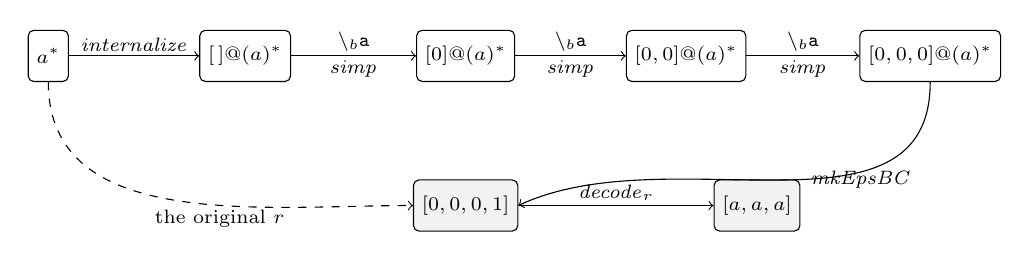
\begin{tikzpicture}[
  expr/.style={draw, rounded corners=2pt, minimum height=6.5mm,
               font=\scriptsize, inner xsep=3pt},
  bits/.style={draw, rounded corners=2pt, minimum height=6.5mm,
               font=\scriptsize, inner xsep=3pt, fill=black!5},
  lbl/.style={font=\scriptsize, inner sep=1.5pt},
]
\node[expr] (r)   at (0,0)    {$a^{*}$};
\node[expr] (ri0) at (2.5,0)  {$[\,]@(a)^{*}$};
\node[expr] (ri1) at (5.3,0)  {$[0]@(a)^{*}$};
\node[expr] (ri2) at (8.1,0)  {$[0,0]@(a)^{*}$};
\node[expr] (ri3) at (11.2,0) {$[0,0,0]@(a)^{*}$};
\node[bits] (bs)  at (5.3,-1.9)  {$[0,0,0,1]$};
\node[bits] (v)   at (9.0,-1.9)  {$[a,a,a]$};

\draw[->] (r)   -- node[lbl, above] {$\mathit{internalize}$} (ri0);
\draw[->] (ri0) -- node[lbl, above] {$\backslash_b \mathtt{a}$}
                   node[lbl, below] {$\mathit{simp}$} (ri1);
\draw[->] (ri1) -- node[lbl, above] {$\backslash_b \mathtt{a}$}
                   node[lbl, below] {$\mathit{simp}$} (ri2);
\draw[->] (ri2) -- node[lbl, above] {$\backslash_b \mathtt{a}$}
                   node[lbl, below] {$\mathit{simp}$} (ri3);
\draw[->] (ri3.south) to[out=-90, in=25]
  node[lbl, right, pos=0.45] {$\mathit{mkEpsBC}$} (bs.east);
\draw[->] (bs) -- node[lbl, above] {$\mathit{decode}_r$} (v);
\draw[->, dashed] (r.south) to[out=-90, in=180]
  node[lbl, below, pos=0.6] {the original $r$} (bs.west);
\end{tikzpicture}
\caption{The bit-coded construction on $a^{*}$ against \texttt{"aaa"}.
Every arrow between expressions points forward, and no
$\mathit{ri}_{i}$ is needed once its successor exists. The expression
stays two nodes wide while the bit-prefix grows by one $0$ per
iteration. The dashed arrow is the one backward dependency left:
$\mathit{decode}$ needs the original $r$ to know what shape the bits
describe.}
\label{fig:single-pass}
\end{figure}

Compare it with Figure~\ref{fig:two-pass}. There the bottom row moves
right to left and needs the whole top row. Here there is no bottom row.
The parse tree is carried along in the annotations, and the two nodes at
the end of the top row are enough to produce it.

Four things have to be defined to make that work: what a bit-string
parse tree is, what an annotated expression is, how the derivative
threads bits through one, and how the bits come back out.

\subsection{Trees as Bit-Strings}
\label{sec:bitcodes}

A parse tree becomes a flat sequence of bits. At an alternation, $0$
marks $\mathit{Left}$ and $1$ marks $\mathit{Right}$. Inside a Kleene
star, $0$ marks "one more iteration" and $1$ marks "stop". A pair of
mutually recursive functions $\mathit{encode}_r$ and
$\mathit{decode}_r$ converts between a $\vdash v : r$ parse tree and its
bit-string.

The star convention is the one place where a bit does not correspond to
an alternation, so it is worth spelling out. Under $r = a^{*}$ the word
$\mathtt{aaa}$ encodes as $[0,0,0,1]$: three $0$s for the three
iterations, then a closing $1$. The empty word under the same $r$
encodes as $[1]$ alone, a star that stops at once.

Two consequences follow. The bit-string's length grows with the number
of iterations and not with the size of $r$. And the bits alone are not a
tree: they record which branch was taken, not what the branches were.
Reading them back needs $r$, which is what $\mathit{decode}_r$ is given.

\subsection{Annotated Expressions}
\label{sec:annotated-expressions}

The idea is to annotate the derivative's \emph{input}, not only its
output. Then, by the time a subexpression has become $\varepsilon$, its
accumulated annotation already is the relevant slice of the final
bit-string.

An annotated expression $\mathit{ri}$ extends $r$ with a bit-list $bs$
at every node except $\emptyset$, which denotes no language and so has
no parse tree to annotate:

\begin{equation}\label{eq:aregex-grammar}
\mathit{ri} \;::=\; \emptyset \mid (bs@\varepsilon) \mid (bs@x) \mid
(bs@\mathit{ri}_1 \oplus \mathit{ri}_2) \mid (bs@\mathit{ri}_1\, \mathit{ri}_2)
\mid (bs@\mathit{ri}^{*})
\end{equation}

Two operations connect the two worlds. $\mathit{internalize}$ converts
$r$ into $\mathit{ri}$ with every bit-list empty, except at an
alternation: the left operand of $r_1+r_2$ is tagged with a leading $0$
and the right with a leading $1$, at construction time. That way a
subtree always carries its own record of which alternative it came from,
with no need to inspect the surrounding structure.

$\mathit{fuse}(bs, \mathit{ri})$ prepends a bit-list onto whatever
annotation $\mathit{ri}$'s top node already carries. Every other
operation here is built from it.

\subsection{The Annotated Derivative}
\label{sec:bderiv-theory}

The derivative is lifted to annotated expressions as
$\mathit{ri} \backslash_b l$. The case structure is
Equation~\eqref{eq:derivative}'s, with bits threaded through instead of
discarded:

\begin{equation}\label{eq:bderiv}
\begin{aligned}
(bs@\mathit{ri}_1 \oplus \mathit{ri}_2) \backslash_b l &=
  (bs@(\mathit{ri}_1 \backslash_b l) \oplus (\mathit{ri}_2 \backslash_b l))
  &&(\mathsf{B}_{+}) \\
(bs@\mathit{ri}_1\, \mathit{ri}_2) \backslash_b l &=
  (bs@(\mathit{ri}_1 \backslash_b l)\, \mathit{ri}_2)
  &&(\mathsf{B}_{\mathrm{seq}}),\ \varepsilon \notin L(\mathit{ri}_1) \\
(bs@\mathit{ri}_1\, \mathit{ri}_2) \backslash_b l &=
  (bs@(\mathit{ri}_1 \backslash_b l)\, \mathit{ri}_2) \oplus
  \mathit{fuse}(\mathit{mkEpsBC}_{\mathit{ri}_1}, \mathit{ri}_2 \backslash_b l)
  &&(\mathsf{B}_{\mathrm{seq}}^{\,n}),\ \varepsilon \in L(\mathit{ri}_1) \\
(bs@\mathit{ri}^{*}) \backslash_b l &=
  (bs@\mathit{fuse}([0], \mathit{ri} \backslash_b l)\; ([\,]@\mathit{ri}^{*}))
  &&(\mathsf{B}_{*})
\end{aligned}
\end{equation}

The concatenation cases mirror the two-way split of
$\mathsf{D}_{\mathrm{seq}}$ and $\mathsf{D}_{\mathrm{seq}}^{\,n}$, with
one addition. On the branch where the derivative abandons
$\mathit{ri}_1$ and jumps into $\mathit{ri}_2$, the bits $\mathit{ri}_1$
would contribute to an empty match are fused onto $\mathit{ri}_2$'s
derivative.

That fusion is the entire optimization. It does immediately, during the
forward pass, what $\mathsf{I}_{\mathrm{seq}}^{R}$ postponed to a later
$\mathit{mkEps}_{r_1}$ call inside $\mathit{inj}$. The work is the same;
the moment is different.

The star case attaches a leading $0$, one more iteration, each time the
body is derived again. The outer $bs$ stays on the new node the rule
produces.

\subsection{Extracting the Bits}
\label{sec:mkepsbc-theory}

$\mathit{mkEpsBC}$ mirrors $\mathit{mkEps}$ but returns bits:

\begin{equation}\label{eq:mkepsbc}
\begin{aligned}
\mathit{mkEpsBC}_{(bs@\varepsilon)} &= bs &&(\mathsf{EB}_{\varepsilon}) \\
\mathit{mkEpsBC}_{(bs@\mathit{ri}_1 \oplus \mathit{ri}_2)} &=
  bs \mathbin{+\!\!+} \begin{cases}
    \mathit{mkEpsBC}_{\mathit{ri}_1} & \varepsilon \in L(\mathit{ri}_1) \\
    \mathit{mkEpsBC}_{\mathit{ri}_2} & \text{otherwise}
  \end{cases}
  &&\begin{array}{l}(\mathsf{EB}_{+}^{L}) \\ (\mathsf{EB}_{+}^{R})\end{array} \\
\mathit{mkEpsBC}_{(bs@\mathit{ri}_1\, \mathit{ri}_2)} &=
  bs \mathbin{+\!\!+} \mathit{mkEpsBC}_{\mathit{ri}_1} \mathbin{+\!\!+} \mathit{mkEpsBC}_{\mathit{ri}_2}
  &&(\mathsf{EB}_{\mathrm{seq}}) \\
\mathit{mkEpsBC}_{(bs@\mathit{ri}^{*})} &= bs \mathbin{+\!\!+} [1] &&(\mathsf{EB}_{*})
\end{aligned}
\end{equation}

The alternation case carries the same left-preference guard as
$\mathsf{E}_{+}^{L}$, and for the same POSIX reason. This is where the
bit-coded construction makes its single decision, and it is the
counterpart of the one \texttt{if} in
Section~\ref{sec:mk-eps-impl}. The star case emits the closing $1$ that
ends a run of iterations.

$\mathit{decode}_r$ then turns the bit-string into an ordinary parse
tree. It takes the original, un-annotated $r$, because the annotated
$\mathit{ri}$ no longer describes the shape being decoded once its own
annotations have been consumed. That is the dashed arrow in
Figure~\ref{fig:single-pass}, and the only thing the construction has to
remember from before the forward pass began.

\subsection{Simplification}
\label{sec:simplification-rules-theory}

Section~\ref{sec:deriv-no-simp} forbade simplification in the direct
construction. The bit-coded construction is under no such restriction,
and it needs one.

The reason it is free to simplify is that the information a backward
pass would need is already carried \emph{on} the expression, as bits.
Replacing $\mathit{ri}_i$ by a smaller expression with the same bits
loses nothing $\mathit{mkEpsBC}$ reads later.

The reason it needs one is growth. \citet{sulzmannlu2014} give the
concrete case

\begin{equation}\label{eq:dp-8}
\begin{aligned}
a^{*} &\xrightarrow{\ a\ } \varepsilon a^{*}
      \xrightarrow{\ a\ } \phi a^{*} + \varepsilon a^{*} \\
      &\xrightarrow{\ a\ } (\phi a^{*} + \varepsilon a^{*})
        + (\phi a^{*} + \varepsilon a^{*})
      \xrightarrow{\ a\ } \cdots
\end{aligned}
\end{equation}

where every step after the first is language-equivalent to
$\varepsilon a^{*}$ and syntactically double the size. Unchecked, this
defeats the point of a single-pass construction, since a growing
$\mathit{ri}$ makes each further $\backslash_b$ step more expensive.

A function $\mathit{simp}$, applied after every derivative step, keeps
the annotated expression small. It propagates $\phi$ through
$\mathit{Seq}$ and $\mathit{Alt}$, flattens and deduplicates nested
alternations keeping the first occurrence of a syntactic duplicate, and
eliminates $\varepsilon$ from a concatenation by
\[
(bs@(bs'@\varepsilon)\, \mathit{ri})
\;\longrightarrow\;
\mathit{fuse}(bs \mathbin{+\!\!+} bs',\ \mathit{ri}),
\]
folding the eliminated node's own bits forward instead of dropping them.
All are instances of Equation~\eqref{eq:simp-identities}, applied to the
annotated grammar and combined with an explicit \emph{isPhi} test. That
test recognizes an empty-language expression built up from these rules,
and not only the literal $\emptyset$ constructor.

\paragraph{Where the bound fails.} On $a^{*}$, $\mathit{simp}$ collapses
every step back to a bit-annotated $a^{*}$, which is exactly
Figure~\ref{fig:single-pass}. That result does not generalize, and it is
worth being precise about the failure instead of letting the $a^{*}$
case stand for the general one. Figure~\ref{fig:simp-growth} measures
node counts per step for two patterns, each with and without
$\mathit{simp}$.

\begin{figure}[ht]
\centering
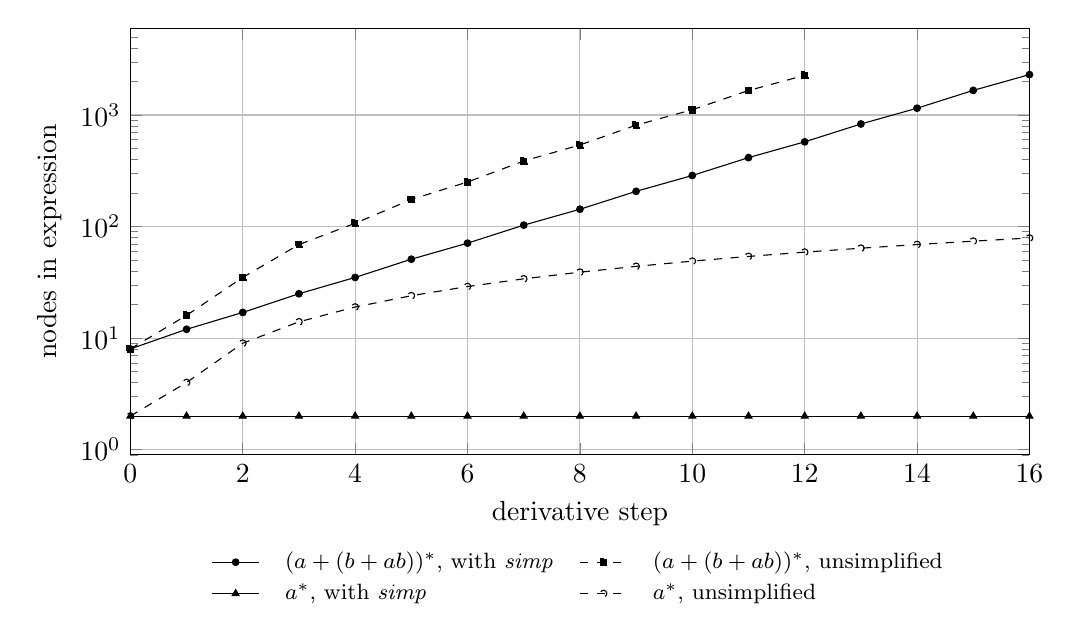
\begin{tikzpicture}
\begin{axis}[
  width=13cm, height=7cm,
  xlabel={derivative step}, ylabel={nodes in expression},
  ymode=log, log basis y=10,
  legend style={at={(0.5,-0.20)}, anchor=north, legend columns=2,
                font=\footnotesize, draw=none, column sep=2.5mm},
  legend cell align=left,
  grid=major, xmin=0, xmax=16, ymax=6000,
]
\addplot[mark=*, mark size=1.2pt] coordinates {(0,8) (1,12) (2,17) (3,25)
  (4,35) (5,51) (6,71) (7,103) (8,143) (9,207) (10,287) (11,415) (12,575)
  (13,831) (14,1151) (15,1663) (16,2303)};
\addlegendentry{$(a+(b+ab))^{*}$, with \emph{simp}}
\addplot[mark=square*, mark size=1.2pt, dashed] coordinates {(0,8) (1,16)
  (2,35) (3,69) (4,107) (5,175) (6,251) (7,387) (8,539) (9,811) (10,1115)
  (11,1659) (12,2267)};
\addlegendentry{$(a+(b+ab))^{*}$, unsimplified}
\addplot[mark=triangle*, mark size=1.4pt] coordinates {(0,2) (1,2) (2,2)
  (3,2) (4,2) (5,2) (6,2) (7,2) (8,2) (9,2) (10,2) (11,2) (12,2) (13,2)
  (14,2) (15,2) (16,2)};
\addlegendentry{$a^{*}$, with \emph{simp}}
\addplot[mark=o, mark size=1.2pt, dashed] coordinates {(0,2) (1,4) (2,9)
  (3,14) (4,19) (5,24) (6,29) (7,34) (8,39) (9,44) (10,49) (11,54)
  (12,59) (13,64) (14,69) (15,74) (16,79)};
\addlegendentry{$a^{*}$, unsimplified}
\end{axis}
\end{tikzpicture}
\caption{Expression size per derivative step, logarithmic vertical
scale. For $a^{*}$, \emph{simp} holds the expression at two nodes while
the unsimplified derivative grows linearly. For $(a+(b+ab))^{*}$ against
$(\mathtt{ab})^{n}$, \emph{simp} reduces the expression substantially at
every step and still leaves it growing exponentially: a straight line on
this scale is exponential growth. Regenerate with
\texttt{cargo run -{}-release -{}-example thesis\_figures -{}- growth};
\texttt{tests/test\_thesis\_figures.rs} pins these values.}
\label{fig:simp-growth}
\end{figure}

The two simplified series behave completely differently. For $a^{*}$ the
line is flat. For $(a+(b+ab))^{*}$ it is straight on a logarithmic axis,
which is to say exponential. Every two characters take the size $s$ to
$2s+1$, so $s+1$ doubles. From $35$ at step 4 the series runs $71$,
$143$, $287$, $575$, $1151$, $2303$ at step 16, and $36\,863$ at step
24. The growth is $\Theta(2^{n/2})$ in the input length.

Two checks rule out the obvious explanations. The figures are unchanged
if the three-way alternation is grouped the other way, as
$((a+b)+ab)^{*}$, which is what the CLI spelling \texttt{"(a|b|ab)*"}
parses to (Section~\ref{sec:regex-syntax}), so the growth depends on the
pattern's shape and not on that grouping. And applying $\mathit{simp}$
repeatedly changes nothing, because a single pass already is the
fixpoint here and produces byte-identical expressions at every step, so
this is not the implementation stopping too early.

The mechanism is specific. Deduplication discards an alternation branch
only when it is \emph{syntactically identical} to an earlier one, and an
annotated branch carries its bit-list as part of its syntax. Counting
the top-level branches of $\mathit{simp}(\mathit{ri}_i)$ at each step,
and counting them again after erasing every annotation, separates the
two:

\begin{center}
\begin{tabular}{lrrrrrr}
\hline
Step & 2 & 4 & 6 & 8 & 10 & 12 \\
\hline
Branches & 2 & 4 & 8 & 16 & 32 & 64 \\
Distinct branches & 2 & 4 & 8 & 16 & 32 & 64 \\
Distinct ignoring bits & 1 & 1 & 1 & 1 & 1 & 1 \\
\hline
\end{tabular}
\end{center}

At every step all of the branches are the same expression structurally.
They differ only in the bits recording which route through the
alternation reached them. So the last row stays at $1$ while the first
two double, and $\mathsf{S}_{4}$ never fires.

The bits are not redundant. Each branch's annotation is a different
candidate parse tree, and $\mathit{mkEpsBC}$'s left-preference is what
selects among them. Dropping duplicates on shape alone would change
which tree the parser returns, and not merely shrink the expression.
That is why the rule is stated on full syntactic equality, and why this
growth is a property of the construction and not a defect in this
transcription of it.

Sulzmann and Lu claim, but do not fully prove, that the construction
runs in time linear in the input. Their grounds are that each of
$\backslash_b$, $\mathit{simp}$, $\mathit{fuse}$, $\mathit{mkEpsBC}$ and
\emph{isPhi} recurses only over subcalls bounded by the now-simplified
expression's size, and they note that detailed space-complexity
estimates are left as future work \citep{sulzmannlu2014}.
Figure~\ref{fig:simp-growth} is one concrete reason that gap matters:
the argument's premise is that $\mathit{simp}$ keeps the expression
small, and that premise holds for $a^{*}$ and fails for
$(a+(b+ab))^{*}$. Chapter~\ref{sec:evaluation} measures the wall-clock
consequence, and Section~\ref{sec:pathological-inputs} returns to this
family.

%

\section{Implementation: \texttt{deriv\_bc}}
\label{sec:derivative-parser-bitcoded-rust}

\subsection{The Annotated Type}
\label{sec:aregex-type}

Equation~\eqref{eq:aregex-grammar} becomes a second enum alongside
\texttt{Regex}, shown in Figure~\ref{fig:aregex-enum}.

\begin{figure}[H]
\begin{verbatim}
#[derive(Debug, Clone, PartialEq, Eq)]
pub enum ARegex {
    Phi,                     // no annotation slot
    Eps(Vec<bool>),          // bs @ eps
    Lit(Vec<bool>, char),    // bs @ l
    Alt(Vec<bool>, Box<ARegex>, Box<ARegex>),
    Seq(Vec<bool>, Box<ARegex>, Box<ARegex>),
    Star(Vec<bool>, Box<ARegex>),
}
\end{verbatim}
\caption{The annotated-expression type, transcribing
Equation~\eqref{eq:aregex-grammar}. Comments are transliterated to
ASCII. \texttt{Phi} is the one variant with no \texttt{Vec<bool>}.}
\label{fig:aregex-enum}
\end{figure}

The grammar's omission of an annotation on $\emptyset$ is enforced by
the type. There is no field to put one in.

Comparing this with Figure~\ref{fig:regex-enum} shows the one place
where a plain \texttt{Regex} will not do. The construction threads
partial parse-tree information through the expression as it is derived,
and that needs somewhere on every node to put it.

The two types also derive different traits, and Rust makes that
difference explicit. \texttt{Regex} derives \texttt{Hash}, because
Chapter~\ref{sec:partial-derivative-parser}'s deduplication uses it as a
\texttt{HashSet} key. \texttt{ARegex} does not, because
\texttt{deriv\_bc} never hashes an annotated expression. Its own
deduplication, inside \texttt{simp}, compares branches pairwise through
\texttt{PartialEq}. A language deriving a fixed bundle of instances at
once would leave that difference implicit.

\subsection{\texttt{internalize} and \texttt{fuse}}
\label{sec:internalize-fuse}

Section~\ref{sec:annotated-expressions} defined two operations on
annotated expressions. Figure~\ref{fig:internalize-rust} gives both.

\begin{figure}[H]
\begin{verbatim}
pub fn fuse(bs: &[bool], ri: ARegex) -> ARegex {
    if bs.is_empty() { return ri; }
    match ri {
        ARegex::Phi => ARegex::Phi,
        ARegex::Eps(p) => ARegex::Eps(combine(bs, p)),
        ARegex::Lit(p, c) => ARegex::Lit(combine(bs, p), c),
        ARegex::Alt(p, r1, r2) =>
            ARegex::Alt(combine(bs, p), r1, r2),
        ARegex::Seq(p, r1, r2) =>
            ARegex::Seq(combine(bs, p), r1, r2),
        ARegex::Star(p, r) => ARegex::Star(combine(bs, p), r),
    }
}

pub fn internalize(r: &Regex) -> ARegex {
    match r {
        Regex::Phi => ARegex::Phi,
        Regex::Eps => ARegex::Eps(vec![]),
        Regex::Lit(c) => ARegex::Lit(vec![], *c),
        Regex::Alt(r1, r2) => {
            let ri1 = fuse(&[false], internalize(r1));
            let ri2 = fuse(&[true], internalize(r2));
            ARegex::Alt(vec![], Box::new(ri1), Box::new(ri2))
        }
        Regex::Seq(r1, r2) => ARegex::Seq(vec![],
            Box::new(internalize(r1)), Box::new(internalize(r2))),
        Regex::Star(r1) =>
            ARegex::Star(vec![], Box::new(internalize(r1))),
    }
}
\end{verbatim}
\caption{\texttt{fuse} prepends a bit-prefix to a node's own
annotation. \texttt{internalize} converts a \texttt{Regex} into an
\texttt{ARegex}, tagging the two sides of every alternation.
\texttt{combine} concatenates the two bit-lists.}
\label{fig:internalize-rust}
\end{figure}

\paragraph{Why it is written this way.}
\texttt{fuse} exists because the annotation lives \emph{inside} every
variant. There is no field common to all of them, so prepending a prefix
means rebuilding the node, which is one arm per variant. \texttt{Phi} is
the exception, and it is the grammar's exception too: it has no
annotation slot, so fusing onto it is a no-op.

The early return is what makes the common case free. \texttt{ri} is an
owned parameter, so \texttt{return ri} is a move and not a copy. The
expression is handed straight back and no node is rebuilt.
\texttt{fuse} runs on every \texttt{Seq} and \texttt{Star} step of every
derivative, and most of those calls carry an empty prefix, so this one
line removes most of the work the function would otherwise do.

\texttt{internalize} is where every bit in the whole construction
originates. Four of its six arms produce an empty \texttt{vec![]}. Only
the \texttt{Alt} arm produces bits, and it produces exactly two, one per
side. That is the concrete content of
Section~\ref{sec:deriv-bc-worked-internalize}'s claim that the
derivative only ever moves bits: no other function in this chapter
introduces a $0$ or a $1$ except $\mathsf{B}_{*}$'s iteration bit and
$\mathsf{EB}_{*}$'s closing bit, both of which are star bookkeeping.

Tagging at construction time, and not at use time, is what removes the
need for a backward pass. A subtree carries its own record of which
alternative it came from, so nothing downstream has to look at the
surrounding structure to find out.

\subsection{The Derivative}
\label{sec:deriv-bc}

Figure~\ref{fig:derivbc-rust} shows the two arms of \texttt{deriv\_bc}
that do something a plain derivative does not.

\begin{figure}[H]
\begin{verbatim}
ARegex::Seq(bs, r1, r2) => {
    if nullable_bc(&r1) {
        let eps_bits = mk_eps_bc(&r1);
        let d1 = deriv_bc(*r1, l);
        let d2 = deriv_bc(*r2.clone(), l);
        let left_branch = ARegex::Seq(vec![], Box::new(d1), r2);
        let right_branch = fuse(&eps_bits, d2);
        ARegex::Alt(bs, Box::new(left_branch),
                        Box::new(right_branch))
    } else {
        let d1 = deriv_bc(*r1, l);
        ARegex::Seq(bs, Box::new(d1), r2)
    }
}

ARegex::Star(bs, r) => {
    let d = deriv_bc(*r.clone(), l);
    let fused = fuse(&[false], d);
    let new_star = ARegex::Star(vec![], r);
    ARegex::Seq(bs, Box::new(fused), Box::new(new_star))
}
\end{verbatim}
\caption{The concatenation and star arms of \texttt{deriv\_bc},
transcribing $\mathsf{B}_{\mathrm{seq}}$,
$\mathsf{B}_{\mathrm{seq}}^{\,n}$ and $\mathsf{B}_{*}$ of
Equation~\eqref{eq:bderiv}.}
\label{fig:derivbc-rust}
\end{figure}

The nullable branch is $\mathsf{B}_{\mathrm{seq}}^{\,n}$ line by line.
\texttt{eps\_bits} is $\mathit{mkEpsBC}_{\mathit{ri}_1}$, computed
\emph{before} \texttt{r1} is consumed by the derivative, and
\texttt{fuse(\&eps\_bits, d2)} carries those bits onto the right branch.

Ownership makes the cost of each branch visible. \texttt{deriv\_bc}
takes \texttt{ri} by value, so in the non-nullable branch \texttt{r2} is
moved into the result and never copied, which matches
$\mathsf{B}_{\mathrm{seq}}$ leaving $\mathit{ri}_2$ untouched. The
nullable branch needs $\mathit{ri}_2$ twice, once underived and once
derived, and \texttt{*r2.clone()} is the deep copy that second use
costs. The star arm is the same story: \texttt{*r.clone()} pays for the
body appearing both derived and underived in $\mathsf{B}_{*}$.

\subsection{\texttt{mk\_eps\_bc} and \texttt{decode}}
\label{sec:mk-eps-bc}
\label{sec:decode}

Figure~\ref{fig:mkepsbc-rust} is Equation~\eqref{eq:mkepsbc}. Read it
next to Figure~\ref{fig:mkeps-rust} and the two are the same function
with \texttt{Vec<bool>} in place of \texttt{ParseTree}.

\begin{figure}[H]
\begin{verbatim}
pub fn mk_eps_bc(ri: &ARegex) -> Vec<bool> {
    match ri {
        ARegex::Eps(bs) => bs.clone(),
        ARegex::Alt(bs, r1, r2) => {
            let mut result = bs.clone();
            if nullable_bc(r1) {
                result.extend(mk_eps_bc(r1));
            } else {
                result.extend(mk_eps_bc(r2));
            }
            result
        }
        ARegex::Seq(bs, r1, r2) => {
            let mut result = bs.clone();
            result.extend(mk_eps_bc(r1));
            result.extend(mk_eps_bc(r2));
            result
        }
        ARegex::Star(bs, _) => {
            let mut result = bs.clone();
            result.push(true);
            result
        }
        ARegex::Phi => panic!("mk_eps_bc called on Phi"),
        ARegex::Lit(_, c) => panic!("mk_eps_bc on Lit('{}')", c),
    }
}
\end{verbatim}
\caption{\texttt{mk\_eps\_bc}, transcribing
Equation~\eqref{eq:mkepsbc}. Each arm starts from the node's own
\texttt{bs} and appends what its children contribute.}
\label{fig:mkepsbc-rust}
\end{figure}

\paragraph{Why it is written this way.}
Every arm opens with \texttt{bs.clone()} and appends to it. That is
$bs \mathbin{+\!\!+} \cdots$ read left to right, and it is why the bits
come out in the order $\mathit{decode}$ expects: a node's own prefix
first, then its children's, in tree order.

The \texttt{Alt} arm is the same \texttt{if} as
Figure~\ref{fig:mkeps-rust}'s, on \texttt{nullable\_bc} instead of
\texttt{nullable}. The two constructions make their one POSIX decision
in the same shape, on the same guard, in functions that share no code.

The \texttt{Star} arm ignores its child entirely, written
\texttt{ARegex::Star(bs, \_)}. A star matching the empty word took zero
iterations, so the body contributes nothing and the only bit to emit is
the closing \texttt{true} of $\mathsf{EB}_{*}$. The underscore makes
that visible in the pattern.

The expression is borrowed here, unlike in \texttt{deriv\_bc}, because
\texttt{mk\_eps\_bc} is called from inside
$\mathsf{B}_{\mathrm{seq}}^{\,n}$ on an \texttt{r1} that the derivative
is about to consume. Reading it without taking it is what lets that rule
compute \texttt{eps\_bits} first and derive afterwards.

\texttt{decode} has no counterpart in the direct construction.
Figure~\ref{fig:decode-rust} gives the two arms that consume the bit
conventions of Section~\ref{sec:bitcodes}.

\begin{figure}[H]
\begin{verbatim}
Regex::Alt(r1, r2) => match bs {
    [false, rest @ ..] => {
        let (v, remaining) = decode_inner(r1, rest);
        (ParseTree::Left(Box::new(v)), remaining)
    }
    [true, rest @ ..] => {
        let (v, remaining) = decode_inner(r2, rest);
        (ParseTree::Right(Box::new(v)), remaining)
    }
    [] => panic!("decode: unexpected end of bits at Alt"),
},

Regex::Star(r1) => {
    let mut iterations = Vec::new();
    let mut remaining = bs;
    loop {
        match remaining {
            [true, rest @ ..] => {
                remaining = rest;
                break;
            }
            [false, rest @ ..] => {
                let (v, after) = decode_inner(r1, rest);
                iterations.push(v);
                remaining = after;
            }
            [] => panic!("decode: end of bits inside Star"),
        }
    }
    (ParseTree::Star(iterations), remaining)
}
\end{verbatim}
\caption{The alternation and star arms of \texttt{decode}. Each arm
returns the tree it built together with the bits it did not use.}
\label{fig:decode-rust}
\end{figure}

Slice patterns make the bit conventions readable as code.
\texttt{[false, rest @ ..]} matches a non-empty slice and binds
\texttt{rest} to everything after the leading bit it has just tested. So
the $0$-means-\texttt{Left} convention is one pattern, and the
$0$-means-another-iteration convention is another.

The helper returns a pair, the tree and the unconsumed remainder,
because decoding a \texttt{Seq} has to hand whatever $r_1$ left over on
to $r_2$. The \texttt{[]} arms assert that a bit-string produced by
$\mathit{mkEpsBC}$ never runs out early, and the public wrapper asserts
that none is left over once the expression has been walked. That is the
same discipline as \texttt{mk\_eps} and \texttt{inject}, at the opposite
end of the construction.

\texttt{decode} takes a plain \texttt{Regex} and a flat
\texttt{Vec<bool>}, which is why it is the one function this chapter
shares with Chapter~\ref{sec:partial-derivative-parser}'s
\texttt{pderiv\_bc}. That parser reaches a \texttt{(Regex, bits)} pair
by an entirely different route and needs the identical final step. It
does not share \texttt{mk\_eps\_bc}, which it reimplements over its own
frontier representation.

\subsection{The Driver}
\label{sec:deriv-bc-driver}

The driver is four lines of loop and three of finish:

\begin{verbatim}
pub fn parse_bitcoded_loop(input: &str, r: &Regex)
    -> Option<ParseTree>
{
    let mut ri = internalize(r);
    for l in input.chars() {
        ri = simp(deriv_bc(ri, l));
    }
    if !nullable_bc(&ri) {
        return None;
    }
    let bits = mk_eps_bc(&ri);
    Some(decode(r, &bits))
}
\end{verbatim}

Compare this with Figure~\ref{fig:deriv-std-drivers-rust}. There is no
\texttt{Vec<Regex>} and no backward loop. The variable \texttt{ri} is
reassigned in place, so only one annotated expression is ever live, and
the \texttt{simp} call is
Section~\ref{sec:simplification-rules-theory}'s requirement applied
after every step.

Note that \texttt{r}, the original expression, is still borrowed at the
last line. That is the dashed dependency of
Figure~\ref{fig:single-pass}, visible in the signature.

%

\section{Worked Example: \texttt{deriv\_bc}}
\label{sec:deriv-bc-worked}

The same $r_1$ against $\mathtt{ab}$, through the other construction,
checked against \texttt{cargo run -- parse "(a|ab)(b|)" "ab" --parser
deriv\_bc --diag 3} (Appendix~\ref{app:report-deriv-bc-match}).

\subsection{Before the Input}
\label{sec:deriv-bc-worked-internalize}

\texttt{internalize} runs first, and the report prints its result:

\begin{verbatim}
ri0 = []@([]@([false]@'a' (+) [true]@([]@'a' . []@'b')) .
  []@([false]@'b' (+) [true]@epsilon))
\end{verbatim}

Read the four tags off. \texttt{[false]} on $a$ and \texttt{[true]} on
$ab$ record the two alternatives of $a+ab$. The same pair appears again
on $b$ and $\varepsilon$. Every other bit-list is empty.

Those four tags are the only bits this expression will ever produce.
Everything that follows moves them; nothing invents new ones.

\subsection{Two Steps}
\label{sec:deriv-bc-worked-forward}

The left operand is not nullable, so the first character takes
$\mathsf{B}_{\mathrm{seq}}$:

\begin{verbatim}
Step 1 (char: 'a', position 1)
  rule: (bs@ri1.ri2) \ 'a'  [nullable_bc(ri1)=false]
       = bs@(ri1\'a'.ri2)
  simp -> []@([]@([false]@epsilon (+) [true]@'b') . []@([false]@'b'
    (+) [true]@epsilon))
\end{verbatim}

Compare against $\mathit{ri}_0$. The literal \texttt{'a'} has become
\texttt{epsilon}, and \texttt{[]@'a' . []@'b'} has become \texttt{'b'}.
Both alternation tags are exactly where they were. One character was
consumed and no bit moved.

The left operand is now nullable, through \texttt{[false]@epsilon}, so
the second character takes $\mathsf{B}_{\mathrm{seq}}^{\,n}$:

\begin{verbatim}
Step 2 (char: 'b', position 2)
  rule: (bs@ri1.ri2) \ 'b'  [nullable_bc(ri1)=true]
       = bs@((ri1\'b'.ri2) (+) (fuse (mkEpsBC ri1) (ri2\'b')))
  simp -> []@([true]@([false]@'b' (+) [true]@epsilon) (+) [false,
    false]@epsilon)
\end{verbatim}

Two bits moved in that step, and both can be traced to their origin.
The \texttt{[false, false]} prefix on the right disjunct is the rule's
\texttt{fuse (mkEpsBC ri1)}: the first \texttt{false} is
$\mathit{ri}_1$'s own empty-match bit, recording that $a+ab$ matched
through its left alternative, and the second is $(b+\varepsilon)$'s
left-alternative tag that it was fused in front of.

The \texttt{[true]} on the left disjunct is new in a different sense. It
tags "the derivative continued into the left operand" as the
$\mathit{Right}$ alternative of the node
$\mathsf{B}_{\mathrm{seq}}^{\,n}$ has just introduced. Where
$\mathit{inj}$ discovered that tagging on the way back, $\backslash_b$
has to commit to it now.

\subsection{Bits to Tree}
\label{sec:deriv-bc-worked-decode}

Both disjuncts of $\mathit{ri}_2$ are nullable, so $\mathit{mkEpsBC}$
faces the choice $\mathit{mkEps}$ faced in
Equation~\eqref{eq:dp-mkeps-derivation}:

\begin{equation}\label{eq:dp-7}
\begin{aligned}
\mathit{mkEpsBC}_{\mathit{ri}_2}
&= [\,] \mathbin{+\!\!+} \mathit{mkEpsBC}_{[1]@(\,[0]@b \,\oplus\, [1]@\varepsilon\,)}
&&\mathsf{EB}_{+}^{L},\ bs = [\,],\ \varepsilon \in L(\mathit{ri}_1) \\
&= [\,] \mathbin{+\!\!+} [1] \mathbin{+\!\!+} \mathit{mkEpsBC}_{[1]@\varepsilon}
&&\mathsf{EB}_{+}^{R},\ bs = [1],\ \varepsilon \notin L([0]@b) \\
&= [\,] \mathbin{+\!\!+} [1] \mathbin{+\!\!+} [1] \;=\; [1,1]
&&\mathsf{EB}_{\varepsilon},\ bs = [1]
\end{aligned}
\end{equation}

The outer step takes $\mathsf{EB}_{+}^{L}$ and the inner one
$\mathsf{EB}_{+}^{R}$, for the same reason in both cases: each rule
tests only its own $\mathit{ri}_1$. At the outer node that is the
$[1]@(\ldots)$ disjunct, which is nullable, so the left branch is taken
and contributes its $bs = [1]$. At the inner node it is $[0]@b$, a bare
literal, which is not, so the right branch is taken and
$[1]@\varepsilon$ contributes the second $1$.

The report confirms the bits and the decode:

\begin{verbatim}
mkEpsBC(ri2) = [11]

decode((a|ab)(b|), [11]):
  = (Right (a, b), Right ())
\end{verbatim}

The two bits select $\mathit{Right}$ at both alternation points of
$r_1$. That is $v_1$ again, the tree Equation~\eqref{eq:dp-inj-a}
reached through an explicit backward pass, read here off the forward
pass alone.

\subsection{The Star Case}
\label{sec:deriv-bc-worked-star}

$r_1$ has no star, so it does not exercise $\mathsf{B}_{*}$ or the
$0$-means-another-iteration convention. Running $a^{*}$ against
\texttt{"aaa"} does, and it is the case Figure~\ref{fig:single-pass}
draws:

\begin{verbatim}
Step 1 ... simp -> [false]@([]@'a')*
Step 2 ... simp -> [false, false]@([]@'a')*
Step 3 ... simp -> [false, false, false]@([]@'a')*

mkEpsBC(ri3) = [0001]
decode(a*, [0001]):
  = [a, a, a]
\end{verbatim}

The expression never changes. It is the two-node
$([\,]@\mathtt{a})^{*}$ at every step, which is $\mathit{simp}$
collapsing $\mathsf{B}_{*}$'s output back to a star. What grows is the
prefix, by one \texttt{false} per character, each one contributed by the
$\mathit{fuse}([0], \ldots)$ in $\mathsf{B}_{*}$. $\mathit{mkEpsBC}$
appends the closing \texttt{true} by $\mathsf{EB}_{*}$, and
$\mathit{decode}$ reads the four bits back as three iterations followed
by a stop.

This is the clearest case for what the construction is for. All of the
parse-tree information is in the prefix and none of it is in the
expression.

%

\section{Comparison}
\label{sec:deriv-worked-example}

Both constructions have now run the same expression against the same
input. Setting the two reports against each other shows the structural
difference in one view. The full reports are
Appendix~\ref{app:report-deriv-std-match} and
Appendix~\ref{app:report-deriv-bc-match}.

\begin{center}
\begin{tabular}{@{}l>{\raggedright\arraybackslash}p{3.9cm}%
                  >{\raggedright\arraybackslash}p{4.3cm}@{}}
\hline
& \texttt{deriv\_std} & \texttt{deriv\_bc} \\
\hline
Report sections & forward, nullability, backward & internalize, forward, nullability, decode \\[2pt]
Named intermediates & \texttt{r0 -> r1 -> r2} & \texttt{ri0 -> ri1 -> ri2} \\[2pt]
Retained at the end & all three & the last one only \\[2pt]
Tree-building calls & 1 \texttt{mkEps} \newline + 2 \texttt{inject} & 1 \texttt{mkEpsBC} \newline + 1 \texttt{decode} \\[2pt]
Simplification & none, by necessity & \texttt{simp} after every step \\[2pt]
Final answer & \multicolumn{2}{@{}l@{}}{\texttt{(Right (a, b), Right ())}} \\
\hline
\end{tabular}
\end{center}

The tree-building row is the one that does not scale with the input.
\texttt{deriv\_std} needs one \texttt{inject} per character.
\texttt{deriv\_bc} needs exactly one \texttt{mkEpsBC} and one
\texttt{decode}, however long the input is. That is the whole content of
the optimization, and it shows in the reports as the difference between
a \texttt{BACKWARD PASS} section whose length depends on the input and a
fixed-size \texttt{MKEEPSBC + DECODE} section.

The final bits \texttt{[11]} and the final tree
\texttt{(Right (a, b), Right ())} encode the same answer. The
correspondence is exact: each \texttt{Right} in the tree is a \texttt{1}
in the bit-string, in the order \texttt{decode} walks the expression.

\paragraph{On a failure.} Run the same $r_1$ against $\mathtt{b}$. That
word is not in $L(r_1)$, since every derivation of $r_1$ must begin by
matching $\mathtt{a}$. Both parsers stop after one derivative step and
neither reaches a tree-building phase. What each holds at that point
differs:

\begin{verbatim}
deriv_std:  r1 = Seq(Alt(Phi, Seq(Phi, Lit('b'))), Alt(Lit('b'), Eps))
              nullable(r1) = false  [FAIL] position 1

deriv_bc:   simp -> phi
            ri1 = phi
              nullable_bc(ri1) = false  [FAIL]
\end{verbatim}

\texttt{deriv\_std}'s expression denotes the empty language but is not
syntactically \texttt{Phi}. It is a \texttt{Seq} whose left operand has
both alternatives dead. \texttt{deriv\_bc}'s \texttt{simp} collapses
that same expression to \texttt{phi}. This is the clearest illustration
of what Section~\ref{sec:simplification-rules-theory}'s \emph{isPhi}
test adds over plain \texttt{simplify}.

Both then report the identical failure, character for character:

\begin{verbatim}
Failure at position:  1 (1-indexed)
Found:                'b'
Expected:             'a'
  b
  ^
\end{verbatim}

The diagnostics layer reads its expected set off the first-literal set
of the expression at the point of failure. It therefore does not depend
on which construction produced that expression, or on how much
simplification was applied to it. This is the pattern across all four
parsers: they differ in what they build on a match, and agree on what
they report when there is nothing to build. The two full failure reports
are Appendix~\ref{app:report-deriv-std-nomatch} and
Appendix~\ref{app:report-deriv-bc-nomatch}.

\paragraph{Agreement.} The two parsers of this chapter, plus
\texttt{deriv\_std}'s loop driver, are three routes to the same tree.
Running all three over 300 randomly generated expressions against 39
inputs each, 11\,700 cases in total, they agree on every one: on whether
the input matched, and on the exact \texttt{ParseTree} returned when it
did. Section~\ref{sec:cross-implementation-equivalence} describes the
generator and the test setup. What matters here is that the bit-coded
route and the inject route share no code beyond \texttt{Regex} itself
and \texttt{nullable}, and are not observed to diverge.

\paragraph{Where this leaves the next chapter.} Both constructions
compute the POSIX tree, and both do it by the same move. Consume the
input with $r\backslash x$, then resolve the one remaining choice, at an
alternation whose two sides both match the empty word, by preferring the
left. The direct construction makes that choice in $\mathit{mkEps}$ on
the way back. The bit-coded one makes it in $\mathit{mkEpsBC}$ at the
end of the way out. Everything else follows from where the choice sits.

Chapter~\ref{sec:partial-derivative-parser} keeps the shape and replaces
$r\backslash x$ with Antimirov's $pd(r,x)$, which returns a \emph{set}.
With a set there is no single expression to be nullable, and no single
alternation to prefer the left of. That turns out to change not only the
machinery but the answer.

%
